%
% Copyright (c) 2024
% Rémy Hubscher - <hubscher DOT remy AT gmail DOT com>
%
% This file may be distributed and/or modified under the terms of 
% the Apache v2 licence
% 

\documentclass{beamer}

\usetheme[shownavigation={false},  % true | false
          utbmlogo={LogoAAA.png},
          logo={logo.png},
          titlepageimage={titleimage.png},
          header=fullnav,          % fullnav | shortnav | utbm
          suiveur={Franck BERTAGNINI},
          dept={Formation FI (A)}
        ]{UTBM}

\usecolortheme{Terra}

\usepackage[francais]{babel}
\usepackage{datetime}  
\usepackage[T1]{fontenc}
\usepackage{lmodern}

\author{Rémy HUBSCHER} 

\begin{document}
  \title[Briefing Long — Prise de Décision Météo]{Prise de décision météo}
  \subtitle{Briefing Long — Prise de Décision Météo}
\date{\today} 

\begin{frame}[plain]
  \titlepage
\end{frame}

\begin{frame}{Objectifs}
  Apprendre à décider suite à une analyse météo :
  \begin{itemize}
    \item de partir en vol \pause
    \item de renoncer au vol
  \end{itemize}
\end{frame}

\begin{frame}{Utilité}
  \begin{itemize}
    \item Voler en toute sécurité ; \pause
    \item Ne pas mettre en danger ses passagers ; \pause
    \item Rester en vie ; \pause
    \item Ne pas se faire peur ; \pause
  \end{itemize}

  \parskip=20pt

  \begin{center}
    « Il y a des pilotes intrédipes et des vieux pilotes,\\
    mais il n'y a pas de vieux pilotes intrépides. »
  \end{center}
\end{frame}

\begin{frame}{Questions}
  \begin{itemize}
    \item Qu'est-ce qu'un METAR ? \pause un TAF ? \pause
    
    \item Qu'est-ce qu'une TEMSI ? \pause une WINTEM ? \pause
    \item Quels sont les outils de prise de météo que vous connaissez ?
  \end{itemize}  
\end{frame}

\begin{frame}{Thème}
  \tableofcontents
\end{frame}

\begin{frame}{Rapport}
  \begin{itemize}
    \item Vous êtes vous déjà dit, j'aurais du rentrer chez moi ? \pause (Averse, neige, grêle)
    \item Avez-vous vu de grosses averses ou orage de grêle ?
    \item Avez-vous fait du vélo par grand vent ?
    \item \href{https://www.youtube.com/watch?v=zIhQlqZ7UN8}{Vidéo tempête dans le Jura}
  \end{itemize}  
\end{frame}

\begin{frame}{Disclaimer}
  Ce briefing long peu se résumer en deux phrases :
  
  \begin{itemize}
    \item Quand il y a un doute, pas de doute, je reste au sol.
    \item Il vaut mieux regretter d'être au sol, que regretter d'être en vol.
  \end{itemize}  
\end{frame}

\begin{frame}{Disclaimer}
  Nous sommes des pilotes privés et rien ne nous oblige à voler.

  En revanche, tout nous oblige à la prudence.

  Nous avons une responsabilité qui a un impact sur de nombreuses
  personnes (famille, ami, aéroclub, propriétaire de l'avion, la société).

  Une analyse sérieuse de la météo est donc nécessaire avant tout vol.

  Elle doit être présente à bord (papier ou numérique).
\end{frame}

\section{Analyse météo à long terme}
\begin{frame}{Analyse météo à long terme}
  \LARGE{Analyse météo à long terme}
\end{frame}

\begin{frame}{Analyse météo à long terme}
  \begin{itemize}
    \item À long terme, on aime avoir une tendance afin de préparer sa nav.\pause
    \item Cela permet de également de choisir un créneau de vol sur la semaine à venir.\pause
    \item Cela permet de donner une tendance à ses passagers sur la faisabilité du vol.
  \end{itemize}
\end{frame}

\subsection{Précipitations}
\begin{frame}{Précipitations}
  Les précipitations sont un indicateur intéressant car elles donnent une information sur :
  \pause
  \begin{itemize}
    \item la visibilité, \pause la nébulosité, \pause les orages.
  \end{itemize}

  \begin{figure}
    \centering
    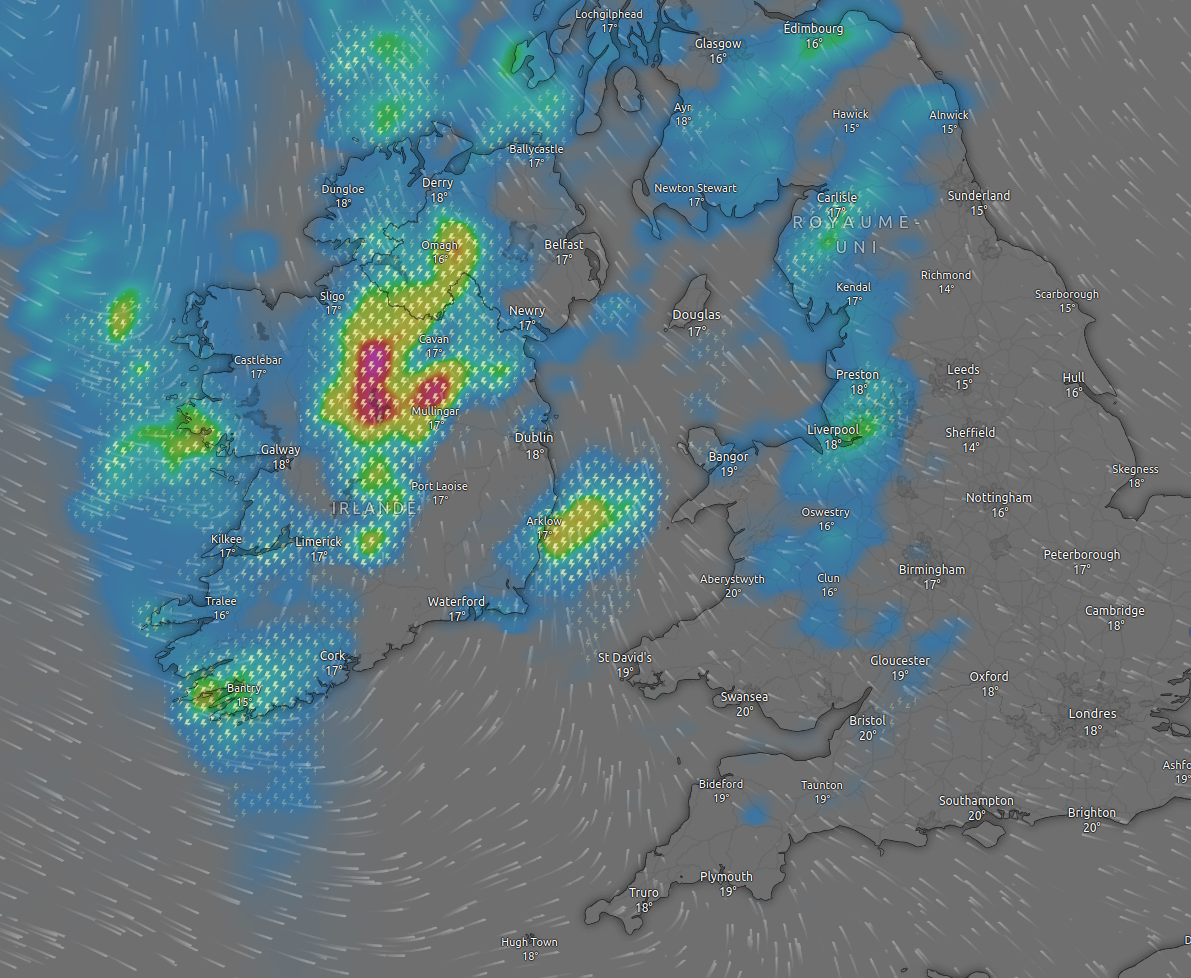
\includegraphics[scale=0.5]{images/windy-rain.png}
  \end{figure}
\end{frame}

\subsection{La base des nuages}
\begin{frame}{La base des nuages}
  La base des nuages donne une information sur la hauteur du plafond.
  \pause
  \begin{itemize}
    \item On évitera de voler avec moins de 2000 ft de hauteur entre le sol et la base des nuages, \pause
    \item Attention au gris qui signifie l'absence d'information : le plafond peut-être au sol. \pause
    \item Il convient de regarder la couverture nuageuses également. \pause
  \end{itemize}

  \begin{figure}
    \centering
    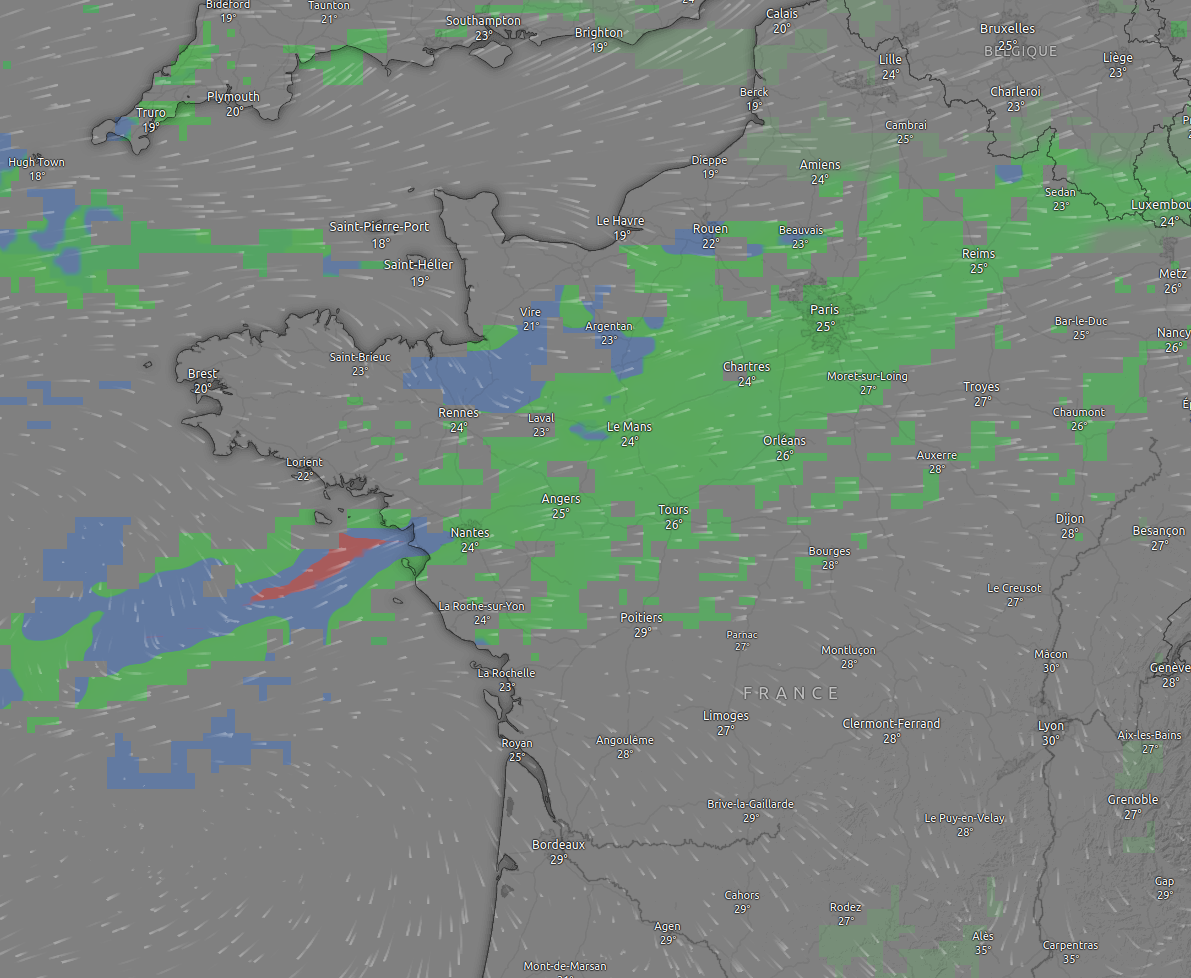
\includegraphics[scale=0.5]{images/windy-base-des-nuages.png}
    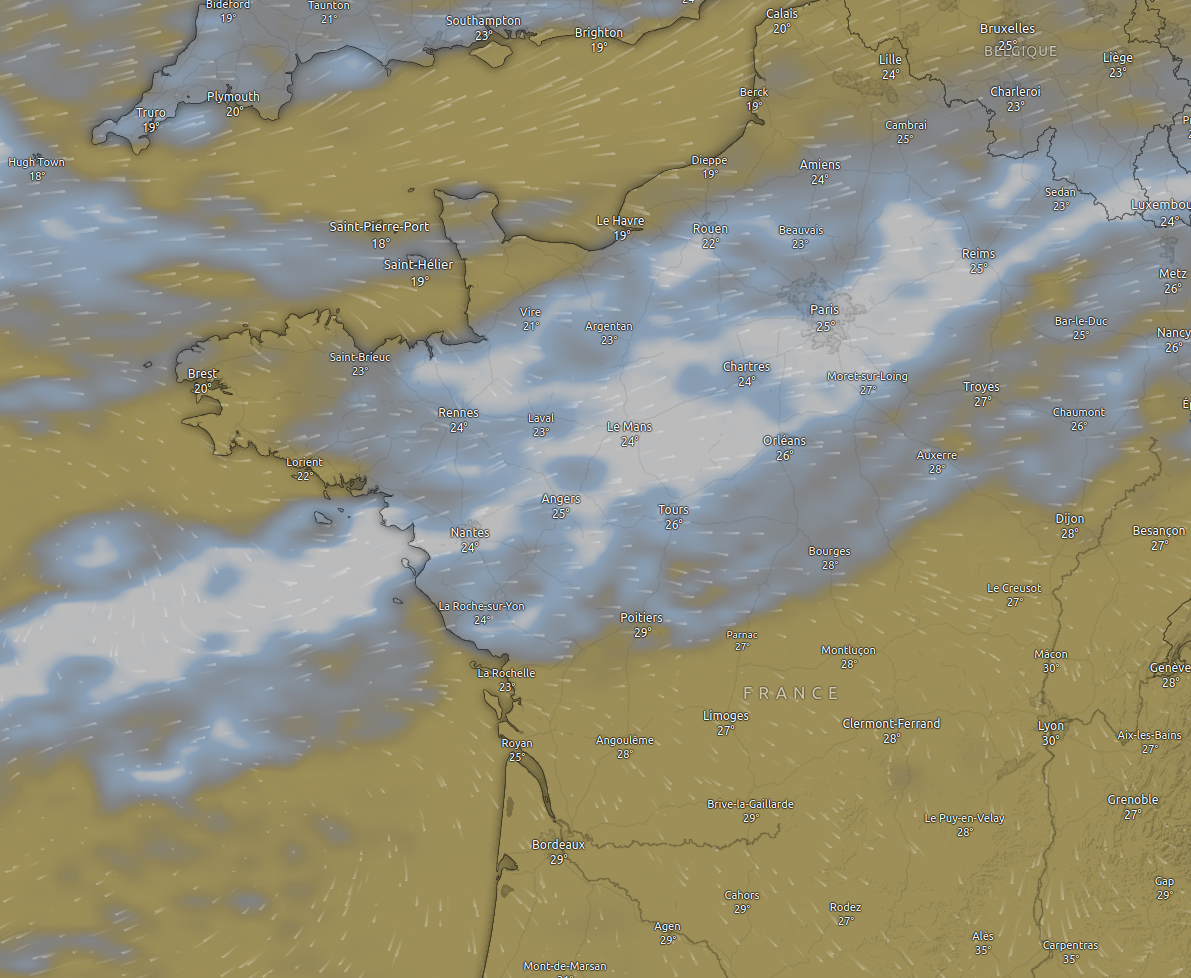
\includegraphics[scale=0.5]{images/windy-clouds.png}
  \end{figure}
\end{frame}

\begin{frame}{Le sommet des nuages}
  Une information intéressante également c'est le sommet des nuages,
  pour savoir si on pourra voler au dessus.
  \begin{figure}
    \centering
    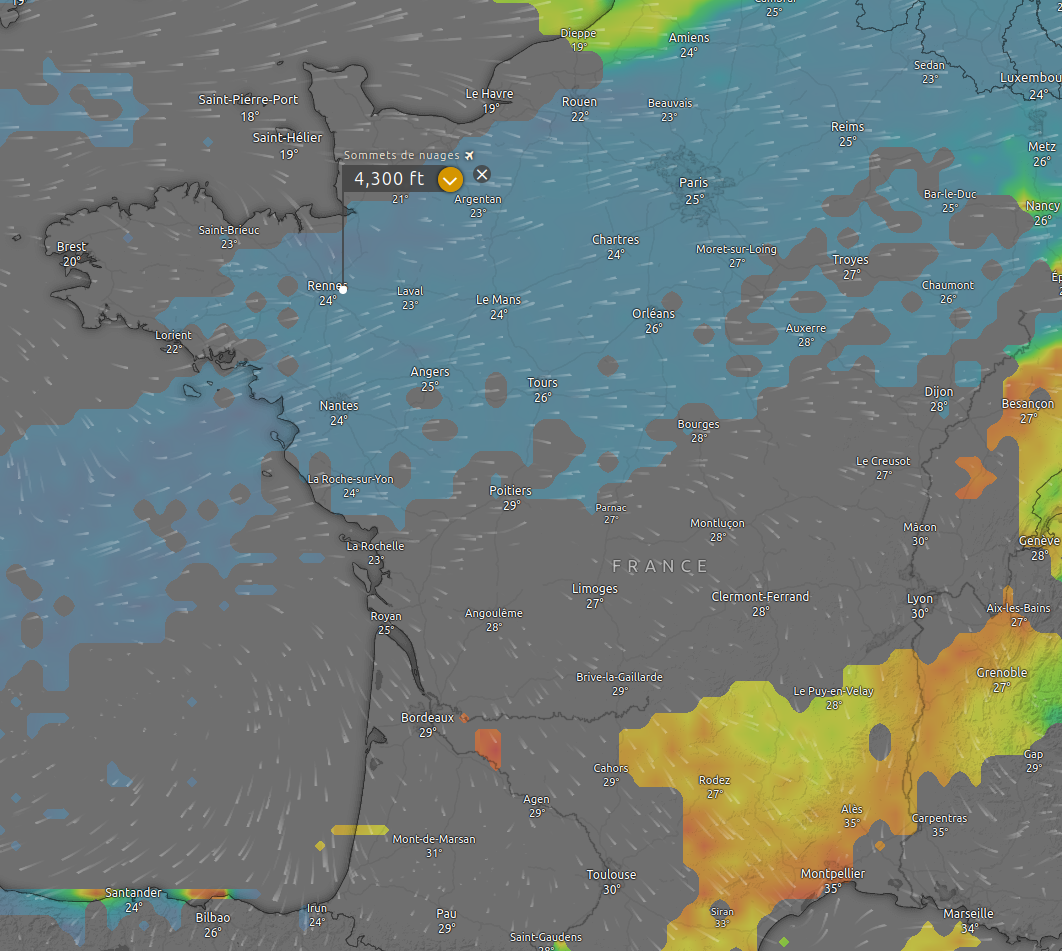
\includegraphics[scale=0.5]{images/windy-cloudtop.png}
  \end{figure}
\end{frame}


\subsection{Brouillard et brûmes}
\begin{frame}{Brouillard et brûmes}
  Brouillards et Brûmes sont les événements les plus difficiles à prévoir à l'avance.
  \pause
  \begin{itemize}
    \item On peut les estimer en comparant la température du point de rosée avec la température ($delta\theta$), \pause
    \item Taux d'humidité (\%) = $100 - delta\theta * 5$ \pause
    \item Base des nuages (ft) = $delta\theta * 420$ \pause
  \end{itemize}

  \begin{figure}
    \centering
    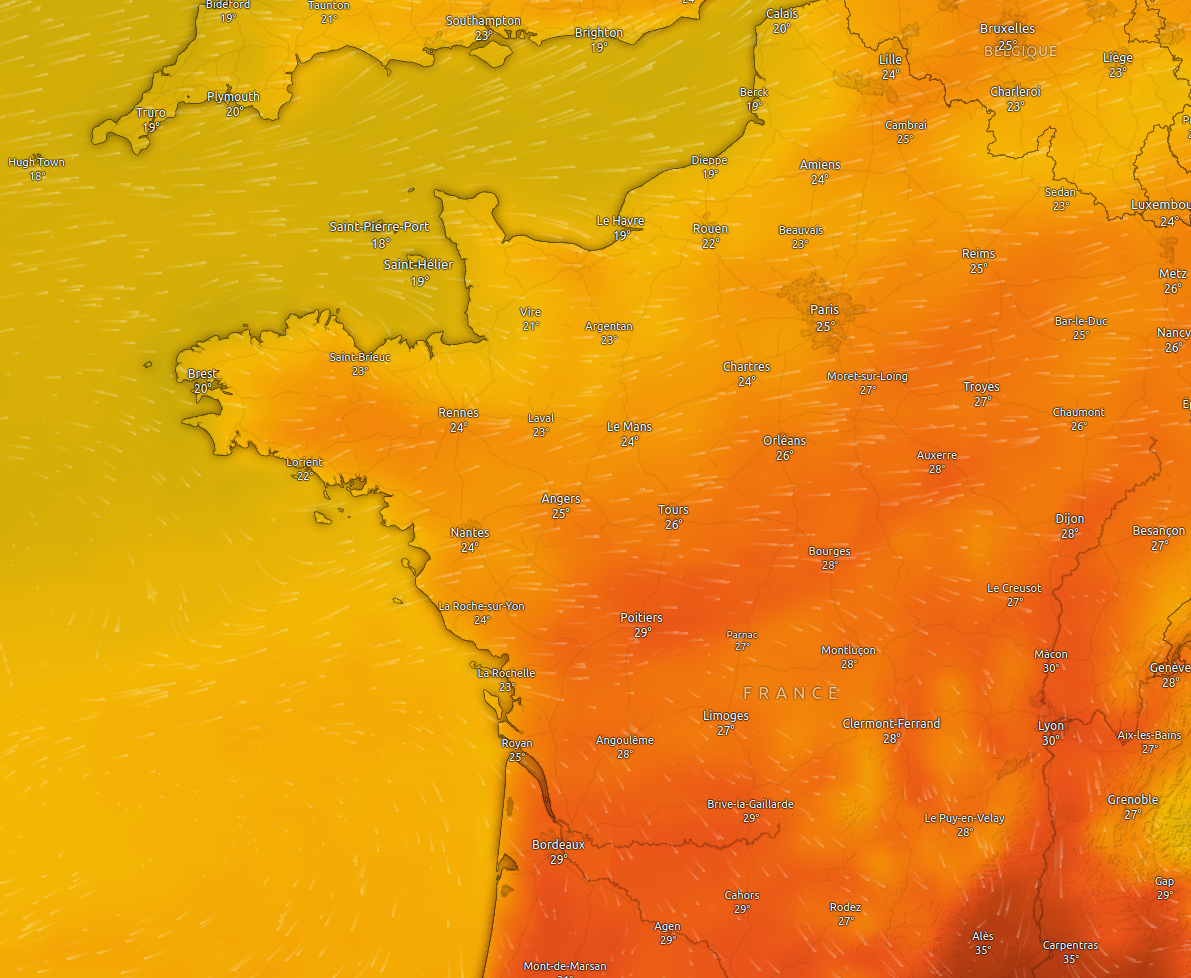
\includegraphics[scale=0.5]{images/windy-temperature.png}
    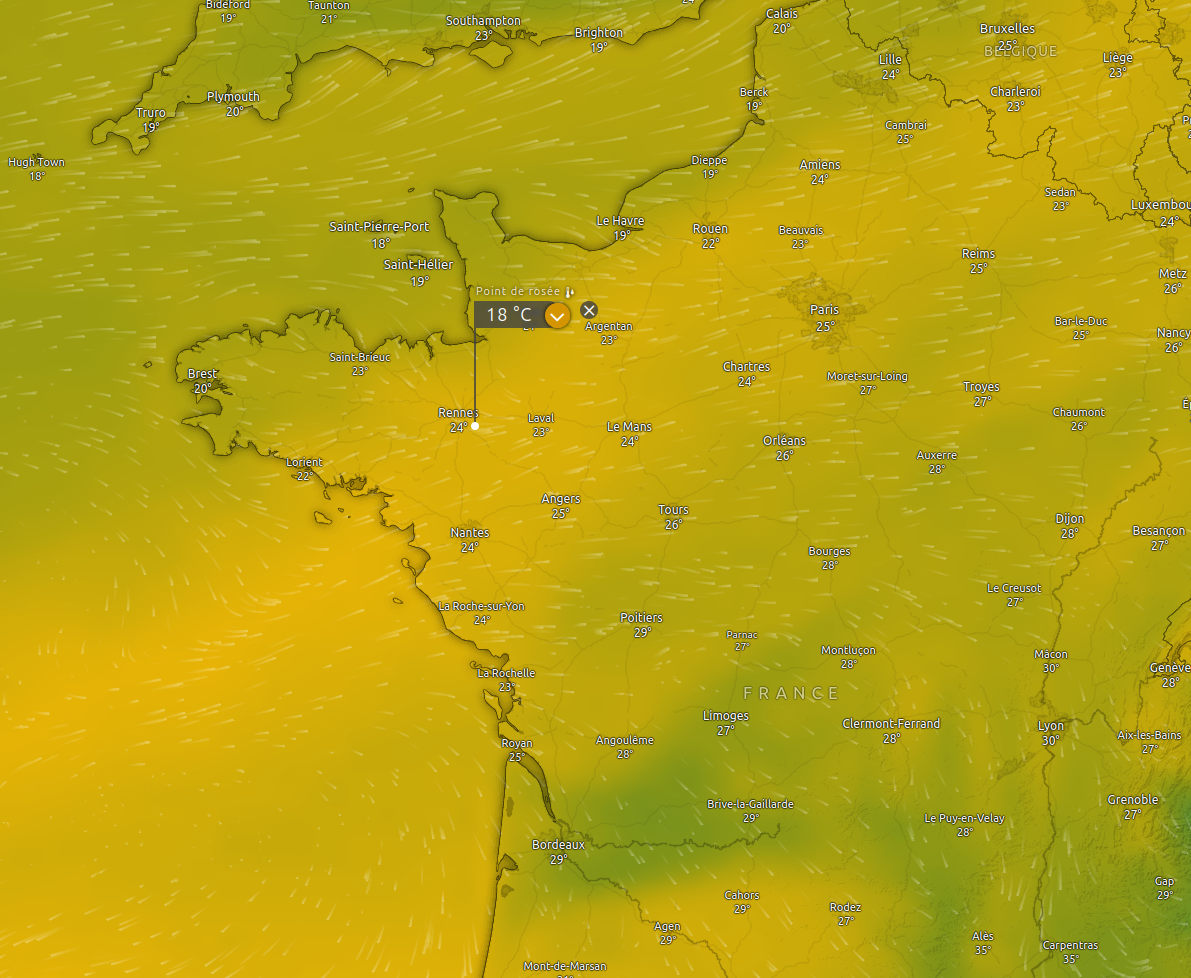
\includegraphics[scale=0.5]{images/windy-point-de-rosee.png}
  \end{figure}
\end{frame}

\begin{frame}{Brouillard et brûmes}
  \begin{itemize}
    \item Température : 24°C \pause
    \item Dewpoint : 18°C \pause
    \item Base des nuages (ft) = 2520 ft \pause
    \item Taux d'humidité = 70\% \pause
  \end{itemize}

  \begin{figure}
    \centering
    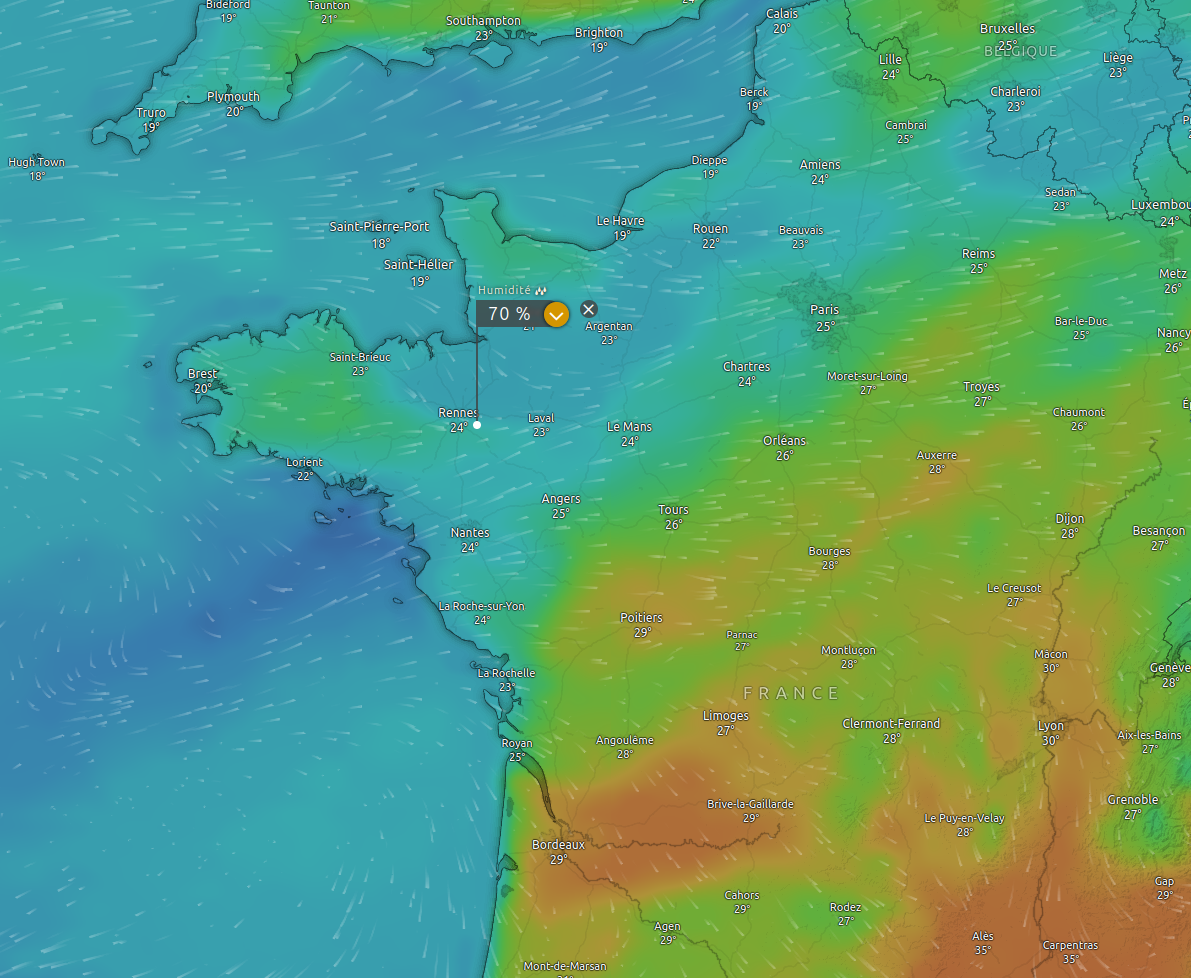
\includegraphics[scale=0.5]{images/windy-humidity.png}
    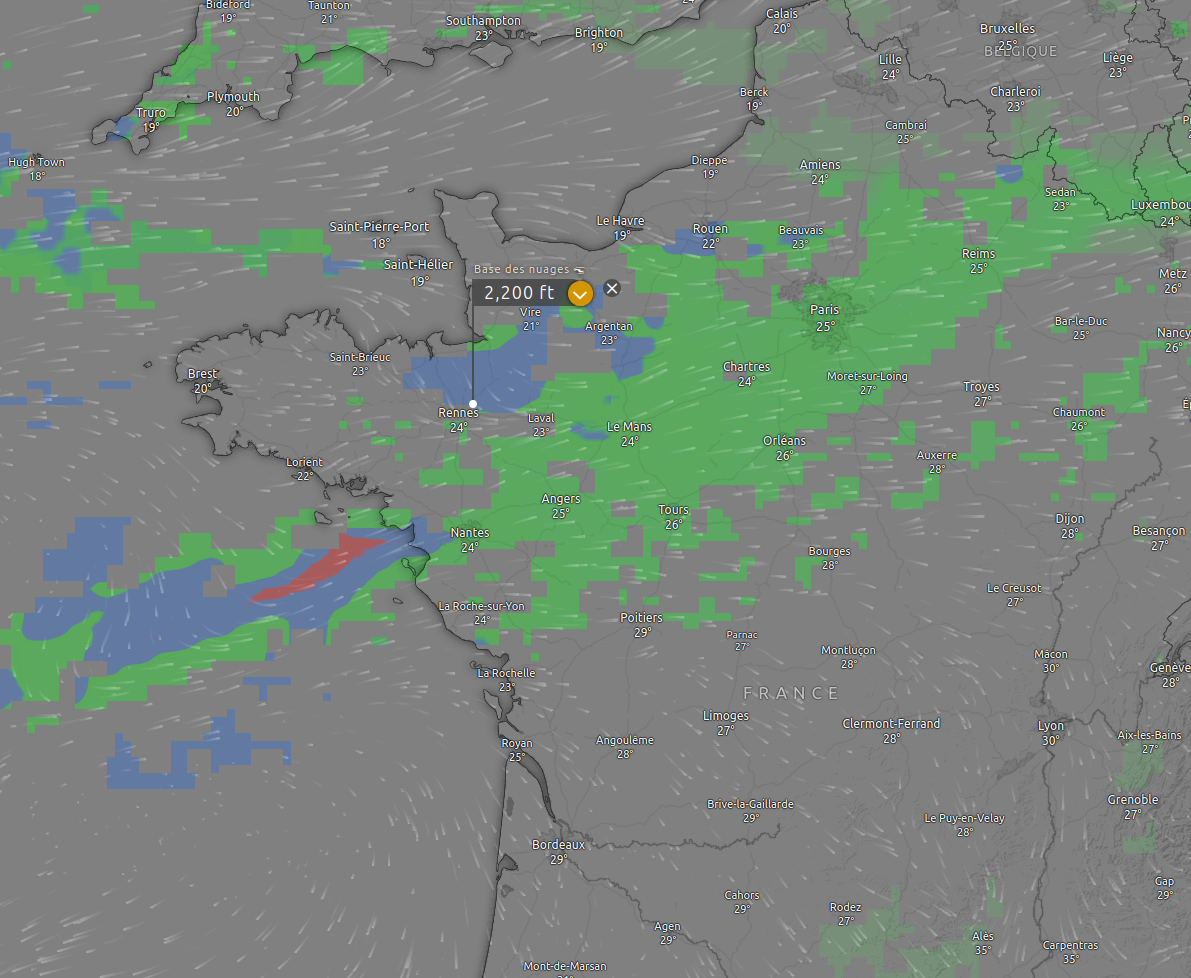
\includegraphics[scale=0.5]{images/windy-cloudbase.png}
  \end{figure}
\end{frame}

\section{Analyse météo à court terme}
\begin{frame}{Analyse météo à court terme}
  \LARGE{Analyse météo à court terme}
\end{frame}

\begin{frame}{Analyse météo à court terme}
  Cette information météo est très appréciable car facile d'accès et visuelle.

  En revanche, ce n'est pas une information aéronautique officielle,
  elle ne peut donc pas se substituer aux informations certifiées.

  Il nous faut donc récupérer le dossier sur aéroweb, actualisé toutes
  les trois heures et publié une heure avant.
\end{frame}

\subsection{METAR / TAF}
\begin{frame}{METAR / TAF}
  Méteo actuelle d'un aérodrôme et prévision sur la journée.
  \pause

  On peut récupérer l'historique des derniers METAR pour analyser
  son l'évolution sur \url{https://aviationweather.gov/}.
  \pause
  \begin{figure}
    \centering
    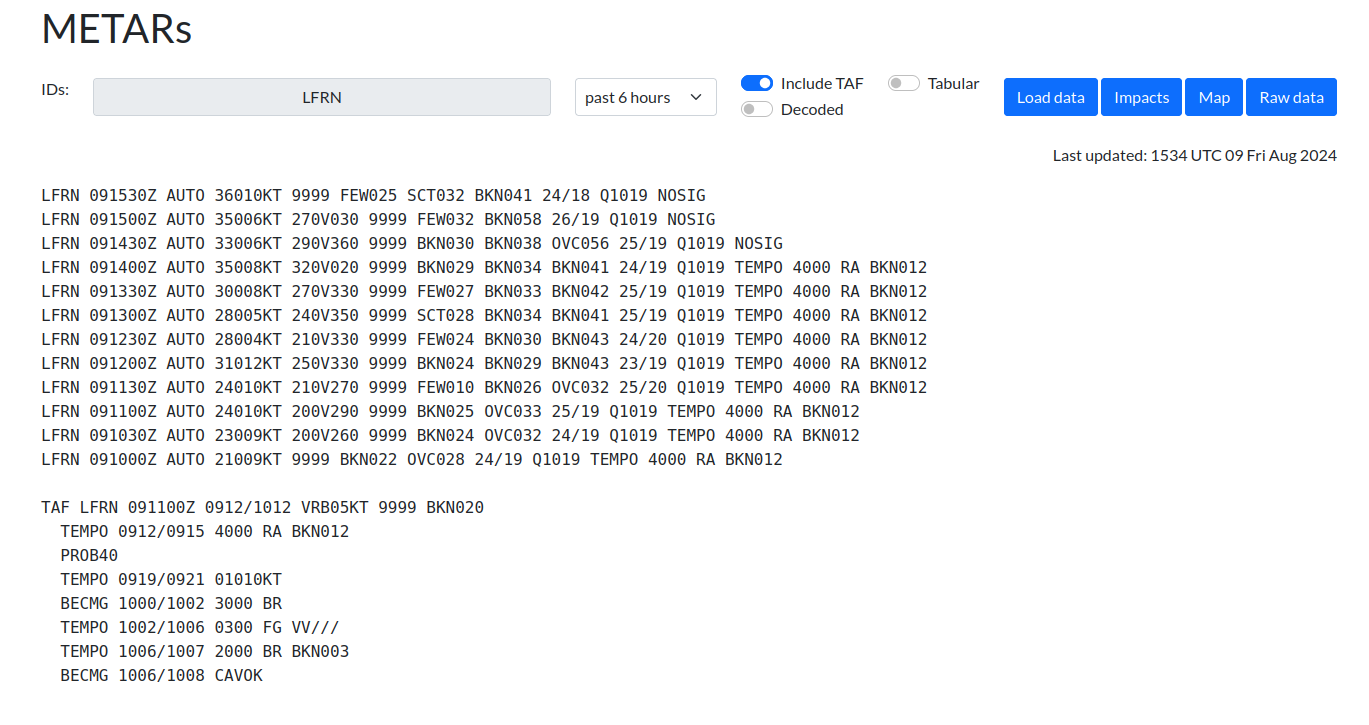
\includegraphics[scale=0.7]{images/aviation-weather.gov.png}
  \end{figure}
\end{frame}

\subsection{TEMSI}
\begin{frame}{TEMSI}
  Temps Significatif sur la France
  \pause
  \begin{figure}
    \centering
    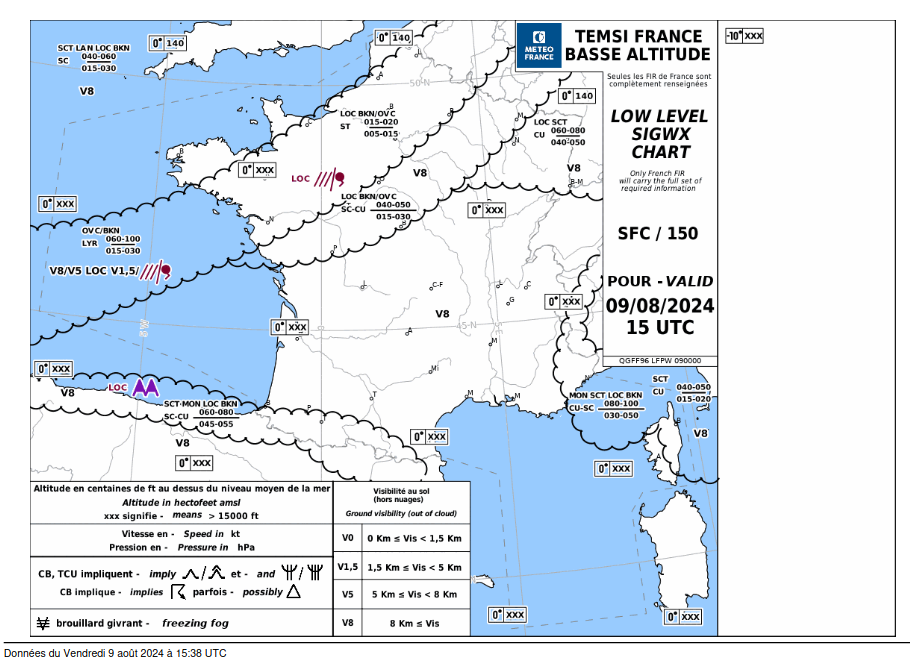
\includegraphics[scale=0.9]{images/temsi.png}
  \end{figure}
\end{frame}

\subsection{WINTEM}
\begin{frame}{WINTEM}
  Vent à différentes altitudes
  \pause
  \begin{figure}
    \centering
    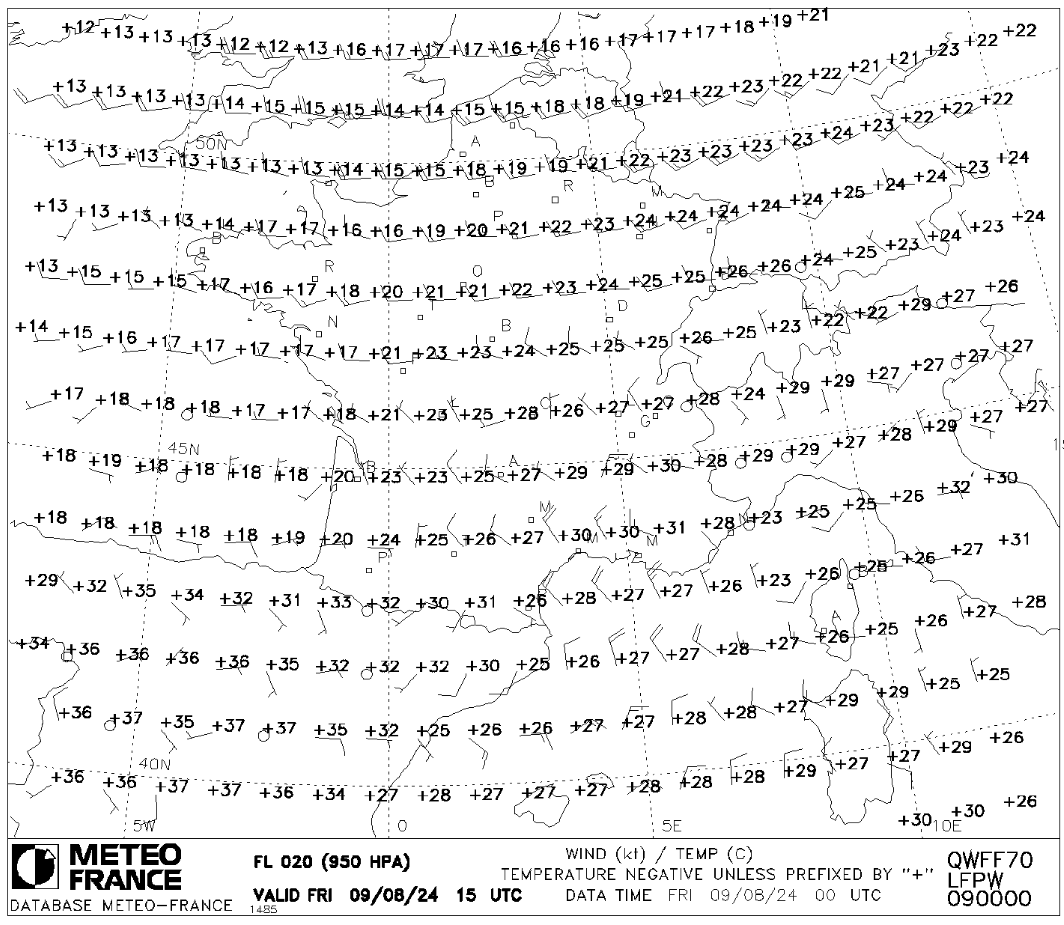
\includegraphics[scale=0.7]{images/wintem.png}
  \end{figure}
\end{frame}

\subsection{Satelite et Radar}
\begin{frame}{WINTEM}
  Précipitations en cours
  \pause
  \begin{figure}
    \centering
    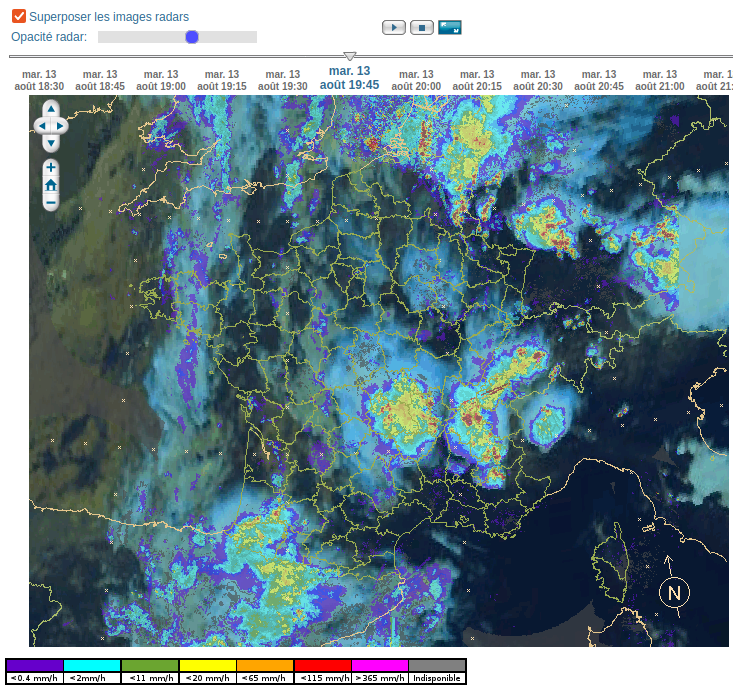
\includegraphics[scale=0.7]{images/satelite.png}
  \end{figure}
\end{frame}

\subsection{SIGMET}
\begin{frame}{SIGMET}
  SIGnificant METeorological Information) : \\Phènomènes météo dangereux
  \pause
  \begin{figure}
    \centering
    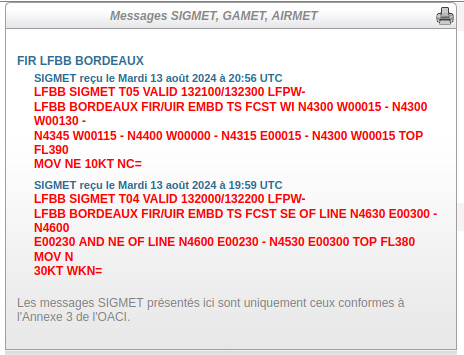
\includegraphics[scale=1.5]{images/sigmet.png}
  \end{figure}
\end{frame}



\section{La prise de décision}
\begin{frame}{La prise de décision}
  Après le recueil de ces données brutes, il convient de les analyser :

  \begin{itemize}
    \item Aérodrôme de destination \pause 
    \item Visibilité
    \item Averses sur le trajet ? \pause 
    \item Composante de vent de travers à l'atterissage ? \pause
    \item Altitude du plus haut point de la route ? \pause
    \item Hauteur de la base des nuages ? \pause
    \item Hauteur du sommet des nuages ? \pause
    \item Temps de vol ?
    \item Vol en montage ? \pause Traversée maritime ? \pause Brûme de mer à l'arrivée ?\pause
    \item Cumuloniumbus ? \pause Orages ? \pause
    \item Givrage ?
  \end{itemize}
\end{frame}

\subsection{Aérodrôme de destination}
\begin{frame}{Aérodrôme de destination}
  L'aérodrôme de destination

  \begin{itemize}
    \item Est-il connu ? \pause
    \item Est-il contrôlé ? \pause
    \item Est-il à fort traffic ? \pause
    \item Quelle est la longueur de la piste ? \pause
    \item Y a-t-il des relief et dangers alentours ? \pause
    \item Y aura-t-il du vent de travers à l'arrivée ? \pause
    \item Y aura-t-il des parachutistes, des planeurs ou de la voltige ?
  \end{itemize}
\end{frame}

\subsection{Météo}
\begin{frame}{Visibilité}
  La visibilité

  \begin{itemize}
    \item $> 10 kms$ ? \pause
    \item $> 8 kms$ ? \pause
    \item $< 5 kms$ ? \pause
    \item Y aura-t-il des averses sur le trajet ?
  \end{itemize}
\end{frame}

\begin{frame}{Nébulositée}
  Les nuages

  \begin{itemize}
    \item Qu'elle est la base des nuages ? \pause
    \item Quel est le sommet des nuages ? \pause
    \item Y a-t-il un risque de brûme ? \pause
    \item Y aura-t-il des orages ou cumulonimbus sur le trajet ? \pause
    \item Y aura-t-il des averses sur le trajet ? \pause
    \item Y a-t-il un risque de givrage ?
  \end{itemize}
\end{frame}

\subsection{Trajet}
\begin{frame}{Le trajet}
  Relief et temps de trajet

  \begin{itemize}
    \item Quel est le temps de vol ? \pause 30 minutes, \pause 1 heures, \pause 2 heures, \pause plus de 2 heures ? \pause
    \item Quelle est l'altitude de sécurité ? \pause Est-elle compatible avec la nébulosité ? \pause
    \item Y a-t-il un survol maritime ? \pause Un vol au dessus des montagnes ? \pause
    \item Y aura-t-il des orages ou cumulonimbus sur le trajet ? \pause
    \item Y aura-t-il des averses sur le trajet ? \pause
    \item Y a-t-il un risque de givrage ? \pause
  \end{itemize}
\end{frame}

\begin{frame}{Le trajet}
  \begin{figure}
    \centering
    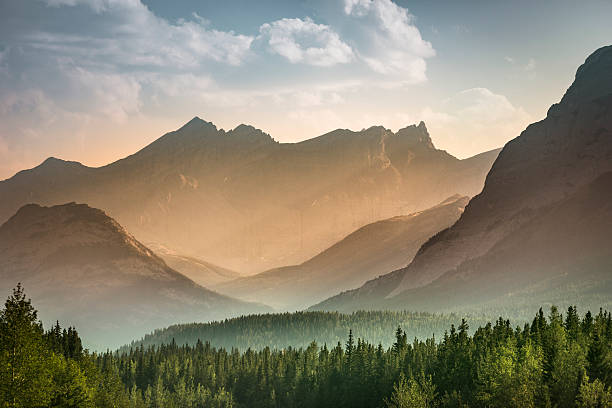
\includegraphics[scale=1.7]{images/montagnes.jpg}
  \end{figure}
\end{frame}


\section{Conclusion}
\begin{frame}{Grille de risque}
  \begin{itemize}
    \item Pour chaque élément, on utilise un code couleur : Vert, Jaune, Rouge. \pause
    \item La décision est simple lorsqu'il y a du rouge. \pause
    \item Lorsqu'il y a du orange, il faut mettre un plan B en face de chaque risque. \pause
    \item L'expérience du pilote sur le trajet, sur le terrain réduit le risque.
  \end{itemize}
  \pause
  \begin{figure}
    \centering
    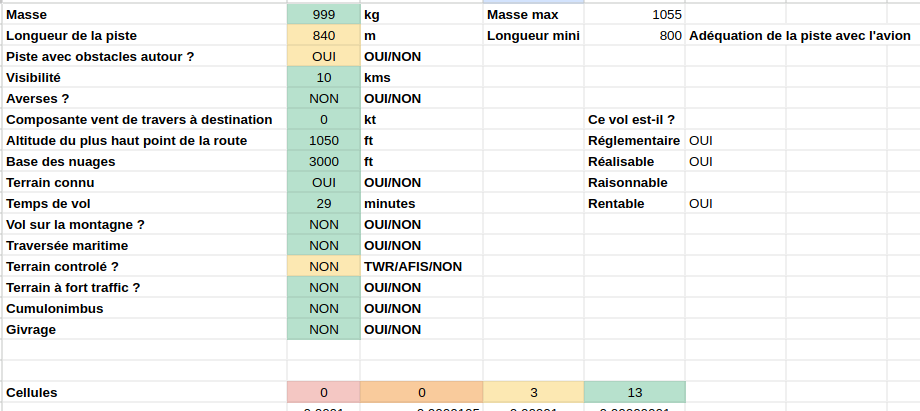
\includegraphics[scale=0.7]{images/tableau-risques.png}
  \end{figure}

\end{frame}

\begin{frame}{Les quatre R}
  Pour aider à la décision, il existe la règle des 4 « R »
  \begin{itemize}
    \item Ce vol est-il réalisable ? \pause
    \item Ce vol est-il réglementaire ? \pause
    \item Ce vol est-il raisonnable ? \pause
    \item Ce vol est-il rentable ? \pause
  \end{itemize}  
\end{frame}

\begin{frame}{Conclusion}
  \begin{itemize}
    \item Ces méthodes nous permettent de prendre la décision avec du factuel. \pause
    \item Il est facile de justifier à ses passagers un report en leur disant qu'on ne souhaite pas mettre leur vie en jeu. \pause
    \item Le plus souvent les passagers comprennent ça comme un gage de sérieux, il faut en être fier.
  \end{itemize}  
\end{frame}

\end{document}
